\section{超自然数和不平等博弈}
    \noindent
    \begin{center}
        \vfill
        \vfill
        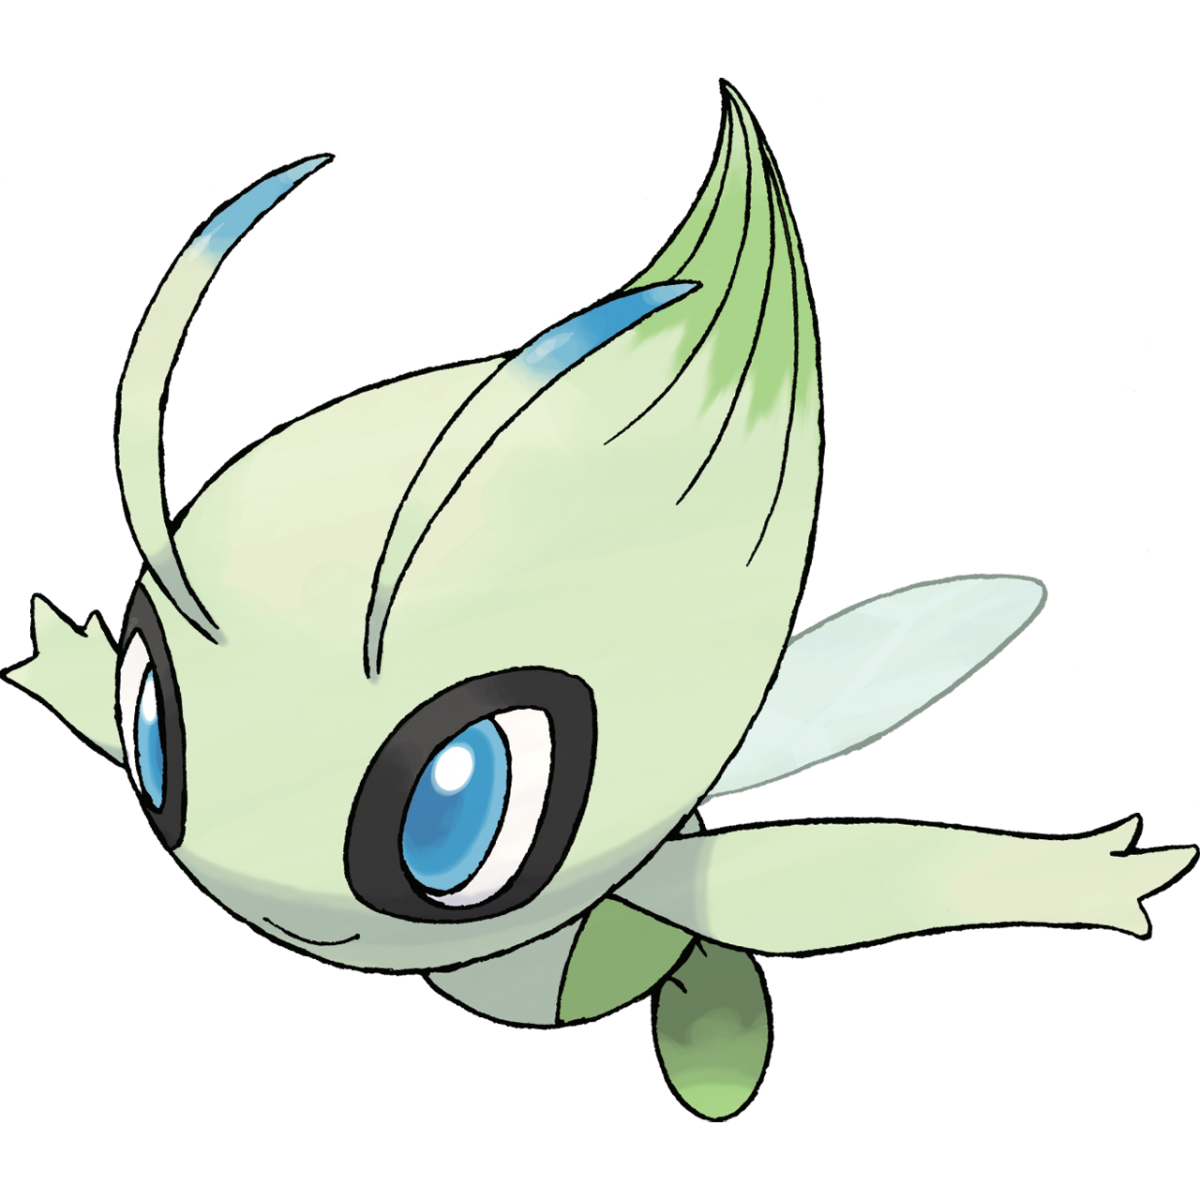
\includegraphics[scale=0.2]{pictures/Celebi.png}
        \vfill
        This page is (maybe un-) intentionally (almost) blank.
        \vfill
    \end{center}
    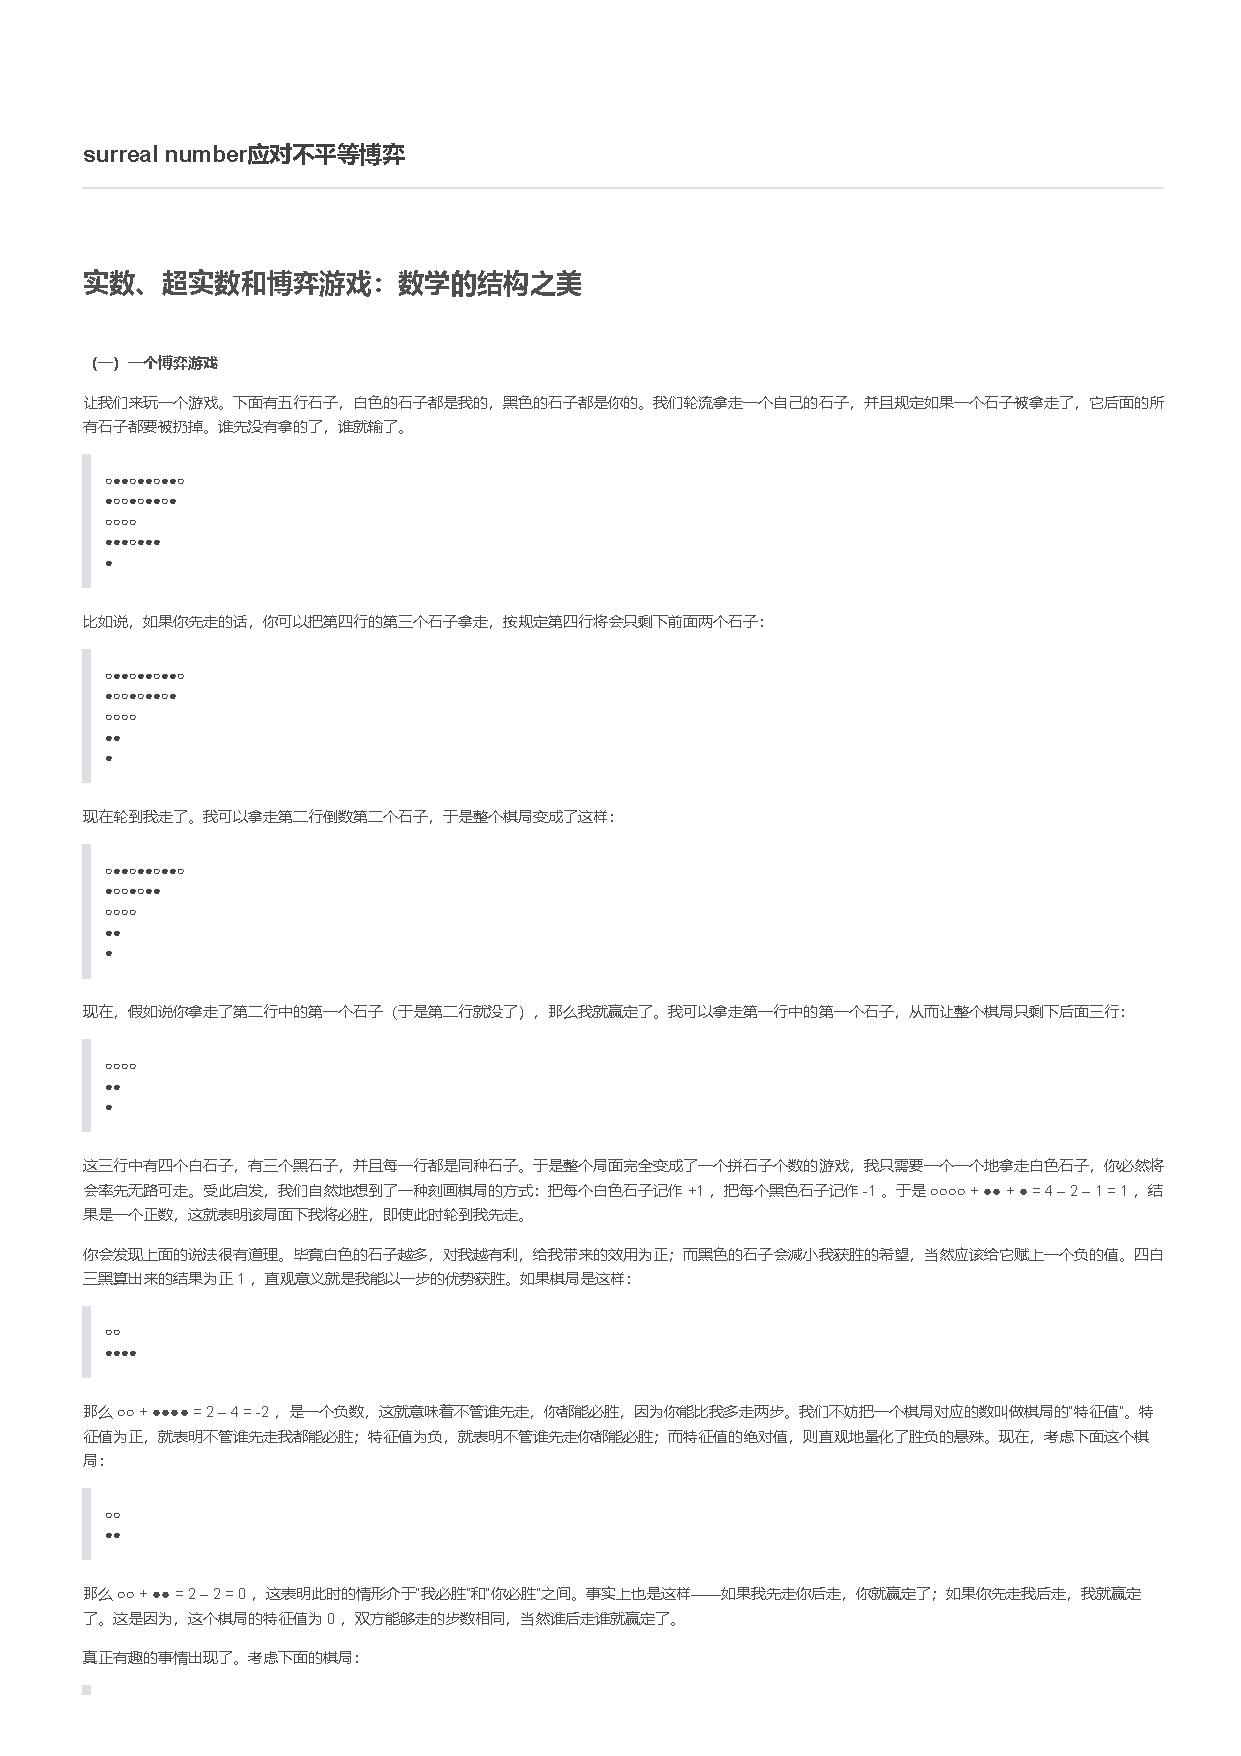
\includepdf[pages=-, scale=0.8, clip, pagecommand={}]{appendix/surreal_number.pdf}

\section{生成函数}
    \noindent
    \begin{center}
        \vfill
        \vfill
        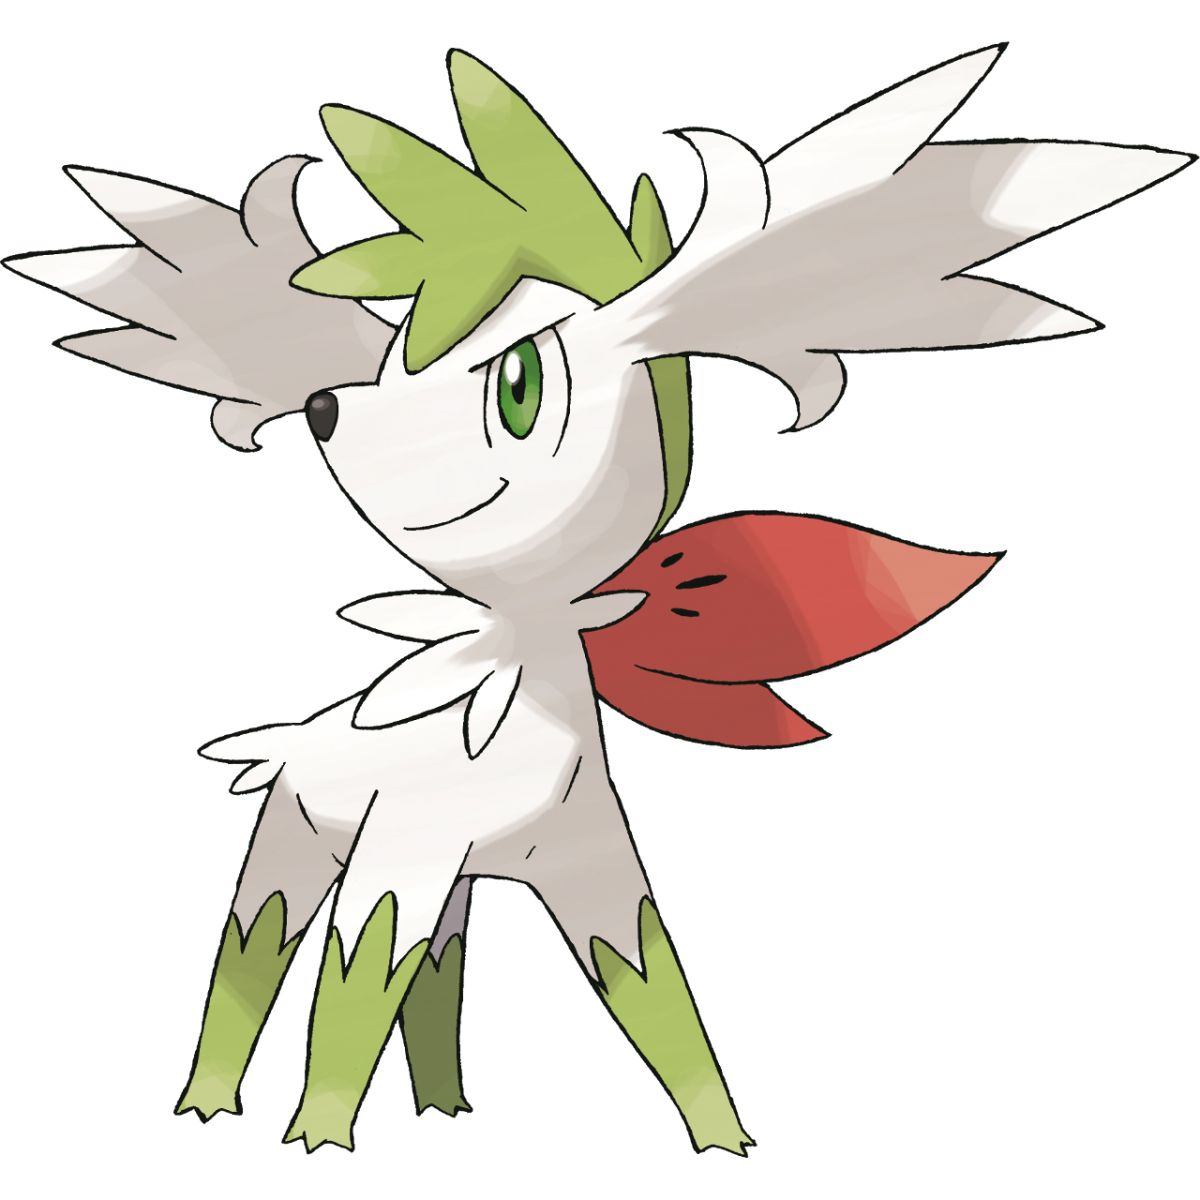
\includegraphics[scale=0.2]{pictures/Shaymin.png}
        \vfill
        This page is (maybe un-) intentionally (almost) blank.
        \vfill
    \end{center}
    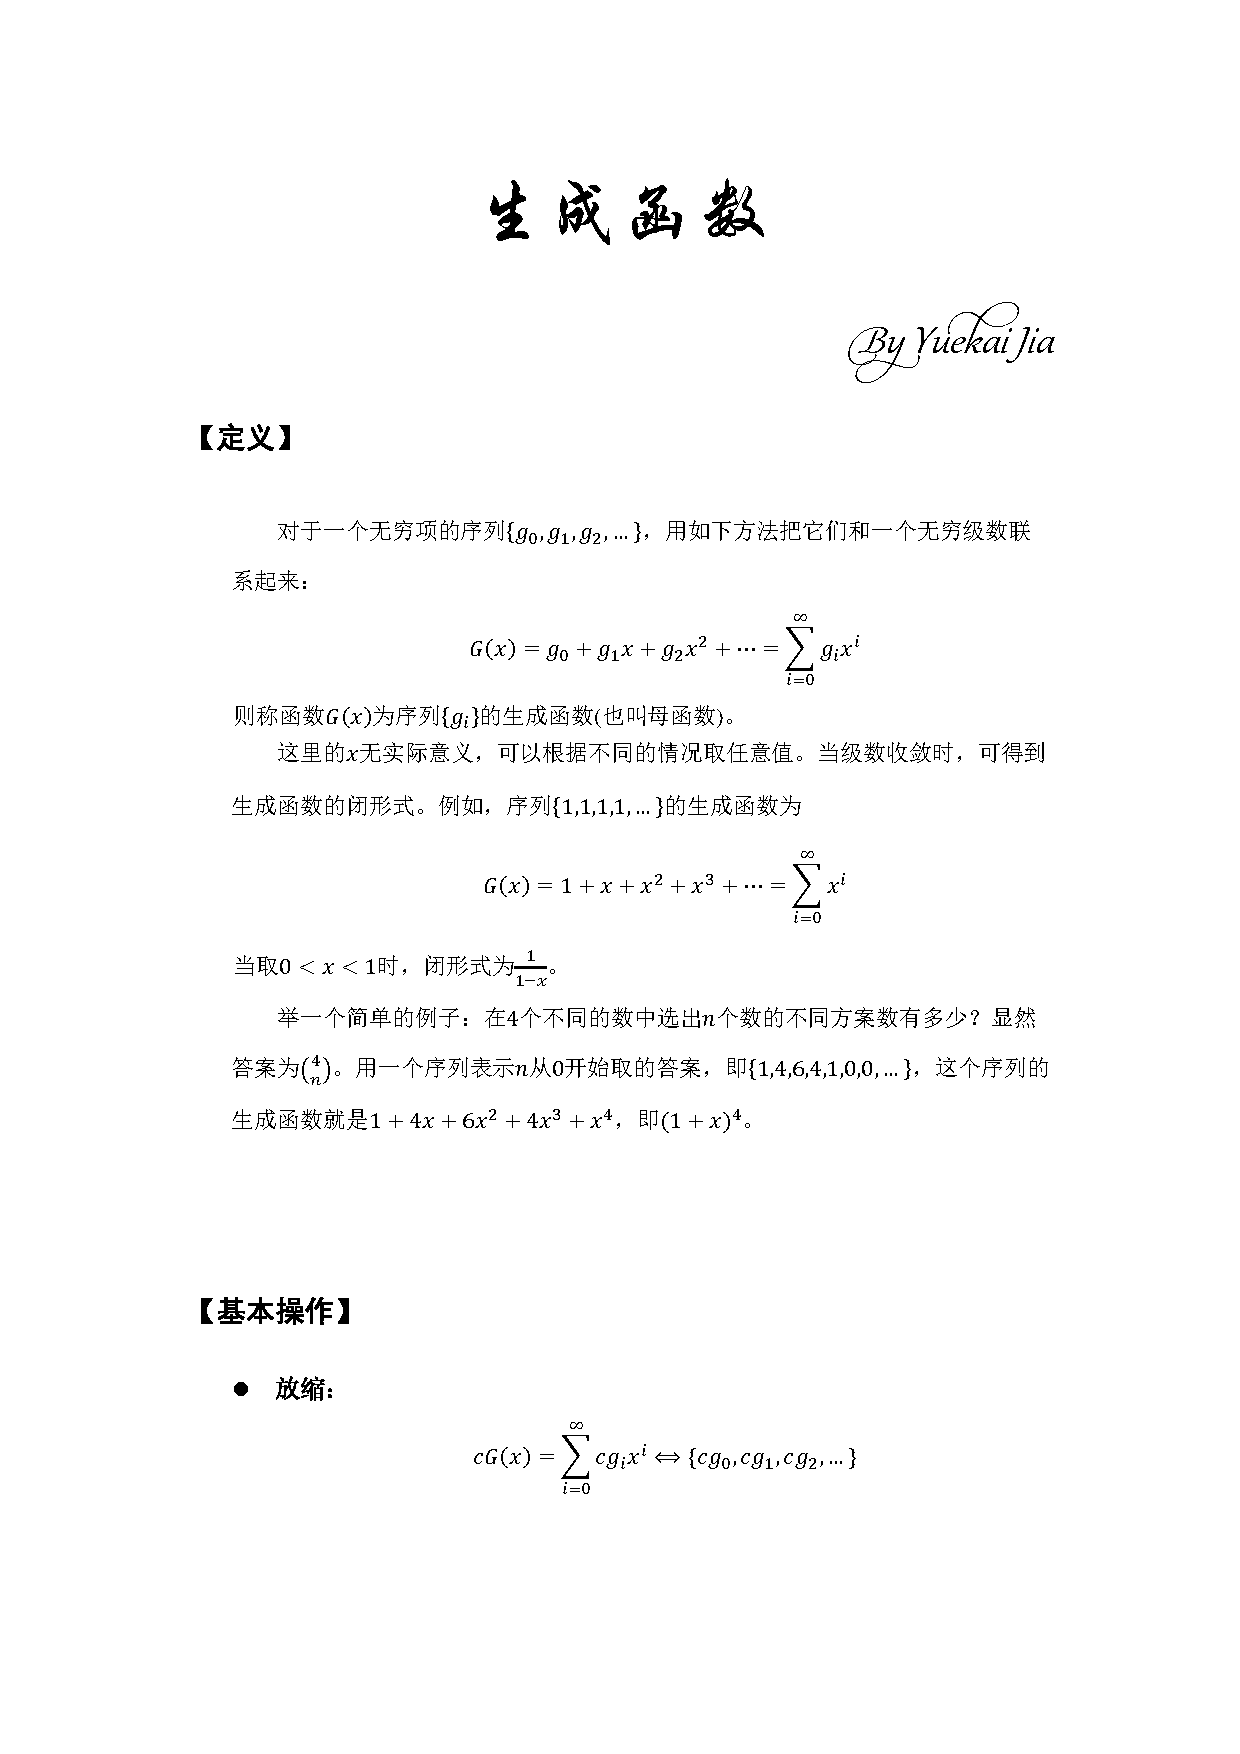
\includepdf[pages=-, scale=0.8, clip, pagecommand={}]{appendix/generator.pdf}

\section{多项式操作}
    \noindent
    \begin{center}
        \vfill
        \vfill
        
\includegraphics[scale=0.2]{pictures/Victini.png}
        \vfill
        This page is (maybe un-) intentionally (almost) blank.
        \vfill
    \end{center}
    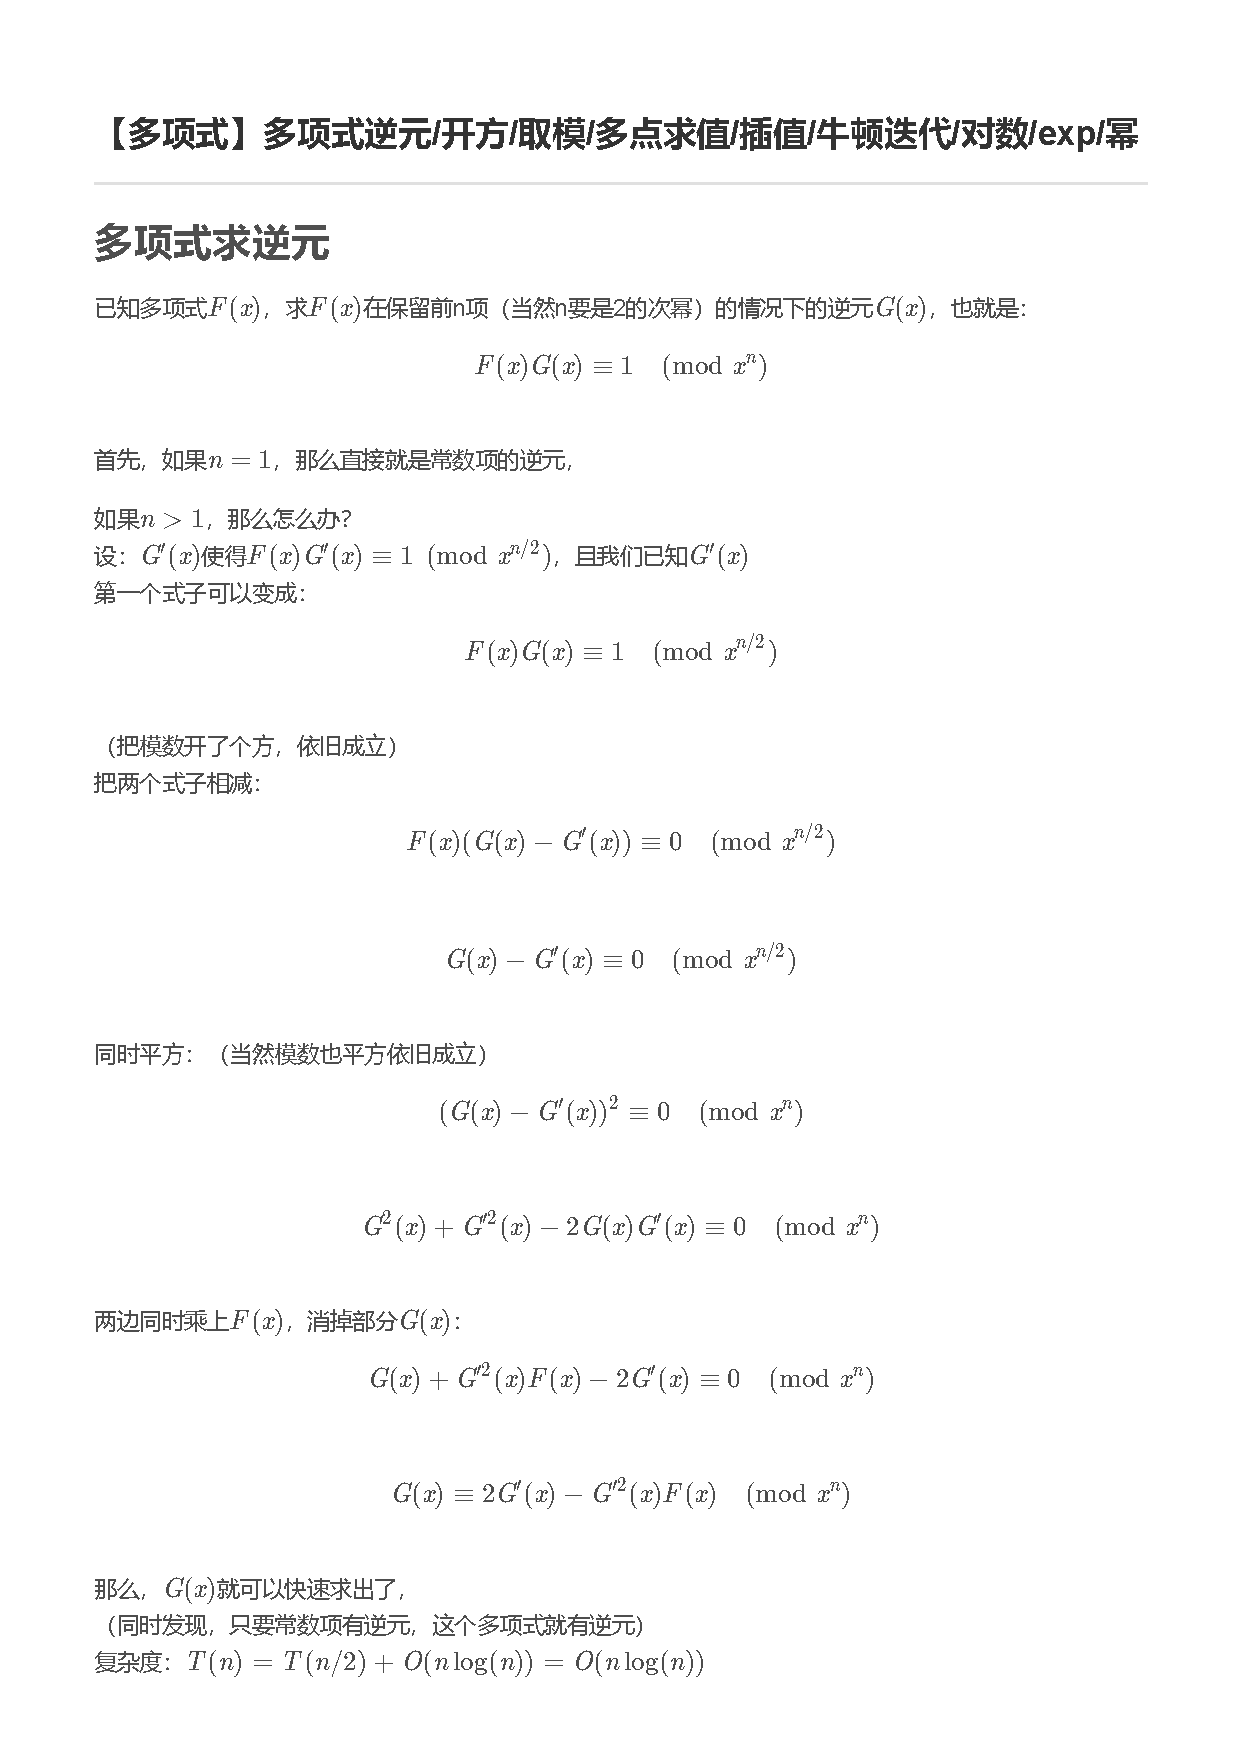
\includepdf[pages=-, scale=0.8, clip, pagecommand={}]{appendix/polynomial.pdf}

\section{多项式操作}
    \noindent
    \begin{center}
        \vfill
        \vfill
        
\includegraphics[scale=0.2]{pictures/Meltan.png}
        \vfill
        This page is (maybe un-) intentionally (almost) blank.
        \vfill
    \end{center}
    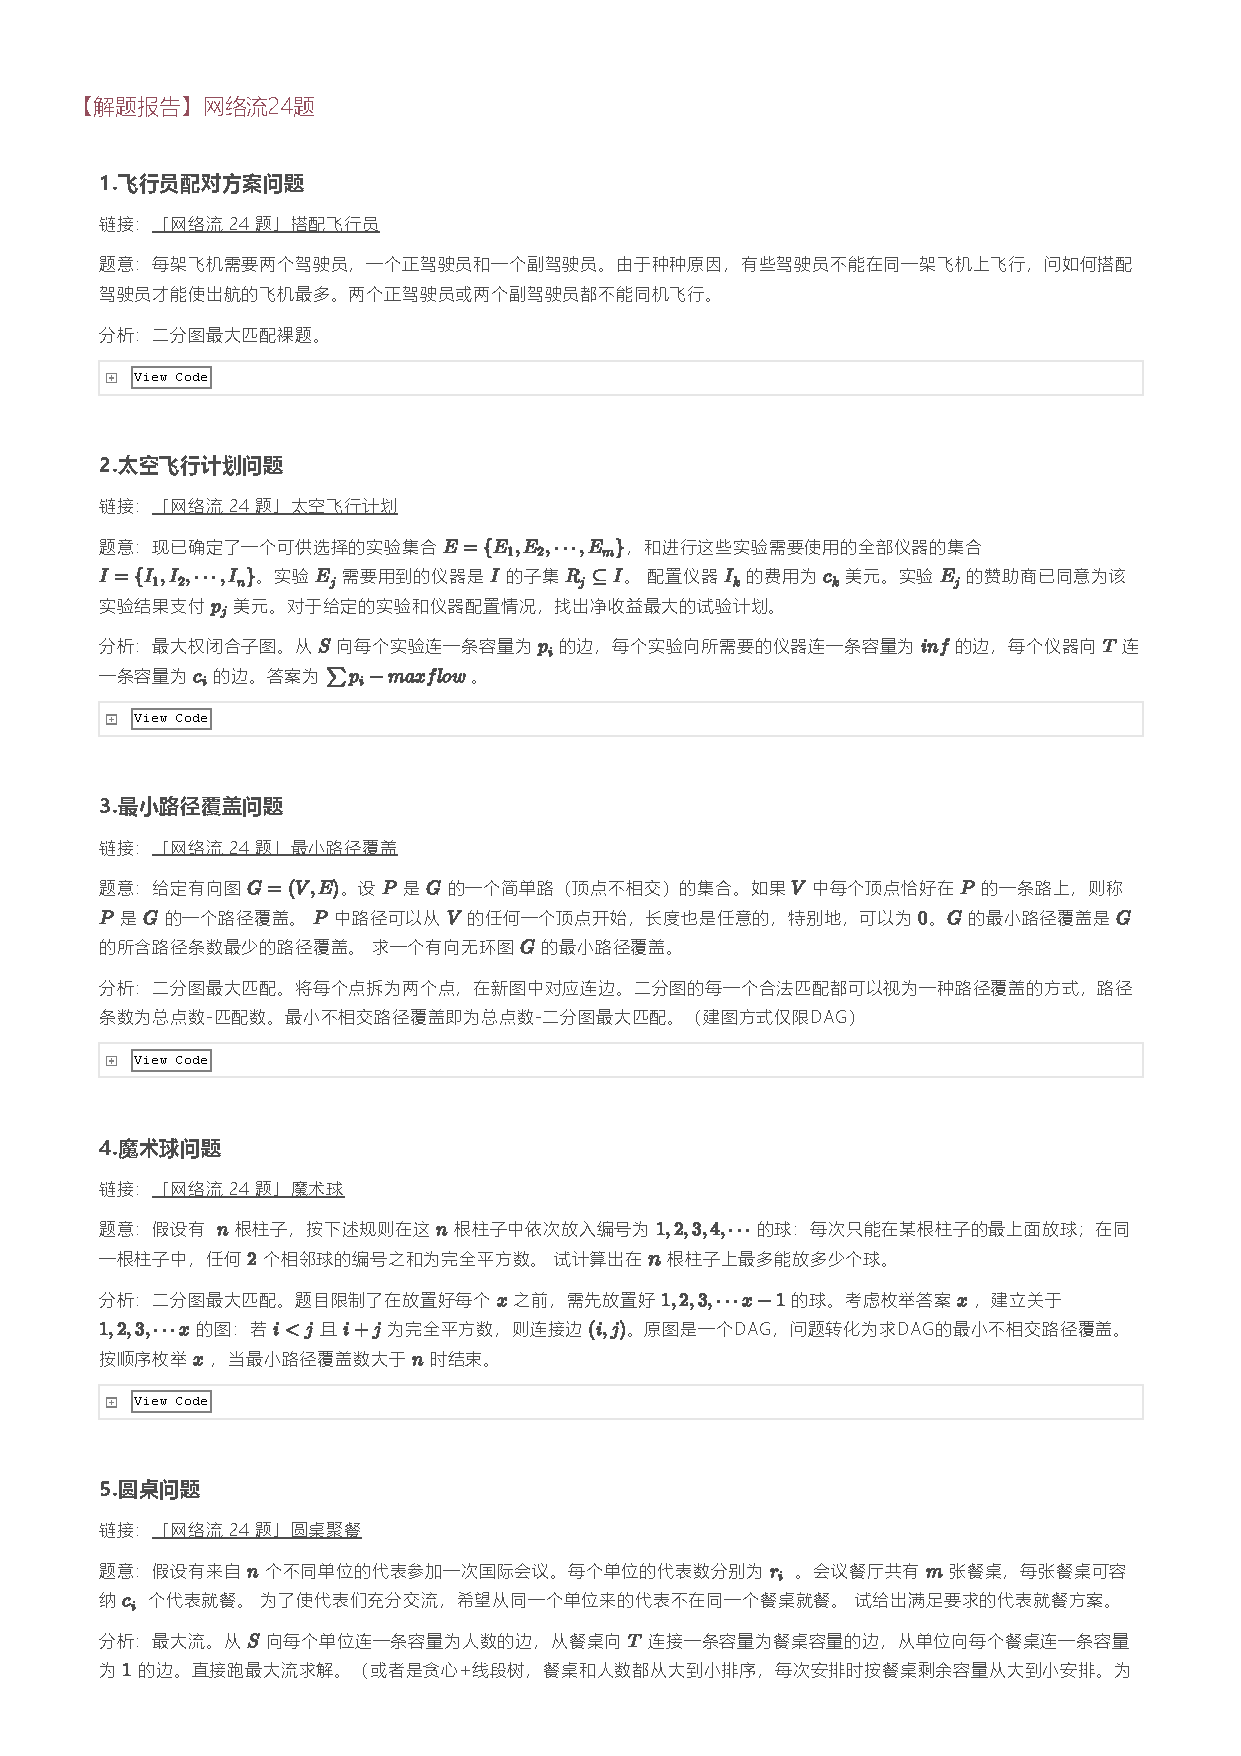
\includepdf[pages=-, scale=0.8, clip, pagecommand={}]{appendix/flow.pdf}

\pagebreak
\hspace{0pt}
\centering
\vfill
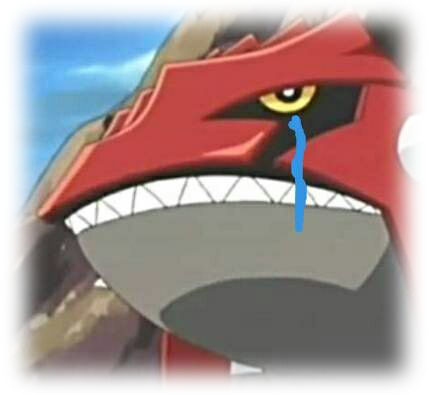
\includegraphics[scale=0.4]{pictures/Groudon.jpg}\\[0.4cm]
------ “还有谁不会飞?” ------
\vfill
\hspace{0pt}
\pagebreak
